\documentclass{article}
\usepackage[utf8]{inputenc}
\usepackage{amsfonts}
\usepackage{graphicx}
\usepackage{pdfpages}
\usepackage{float}

\graphicspath{ {./figures/} }

\title{Mini Projet Data Science}
\author{HAJAGE Michael, RODRIGUES PEREIRA Lucas et PONT Mathieu}
\date{Mai 2019}

\begin{document}

\maketitle

\section{Introduction}
Dans le cadre de la première année du master informatique de l'université de Paris (anciennement Paris Descartes) il nous a été demandé dans le cours "Data Science" de réaliser un projet utilisant le jeu de données Fashion-MNIST. 

Nous devons analyser ce jeu de données à l'aide des différents algorithmes suivants:

\begin{itemize}
\item Principal Component Analysis (PCA)
\item t-distributed Stochastic Neighbor Embedding (t-SNE)
\item Autoencoder
\item K-Means
\item Support Vector Machines (SVM)
\item Linear Discriminant Analysis (LDA)
\end{itemize}

\section{Principal Component Analysis (PCA)}

Nous avons commencé par l'analyse en composantes principales (en utilisant R et le package \textit{FactoMineR}) dont les deux premières composantes n'expliquent que 46.8\% de la variance totale des données. La troisième composante (non représentée sur les différentes figures) n'apporte que 6\% d'inertie.

Etant donné que chaque variable sont dans un intervalle identique nous avons décidé de faire une ACP non normée, avec une ACP normée nous n'avons que 36.49\% d'inertie.

On voit sur le plan factoriel des variables (figure \ref{fig:pca_var})

\begin{figure}[H] 
\centering
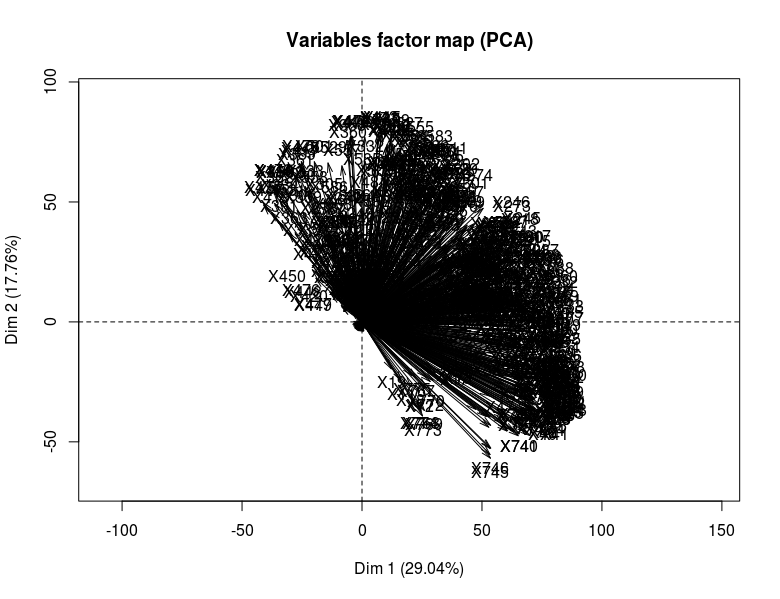
\includegraphics[width=300]{pca_var_factor_map.png}
\caption{Plan factoriel des variables avec PCA.}
\label{fig:pca_var}
\end{figure}

\begin{figure}[H] 
\centering
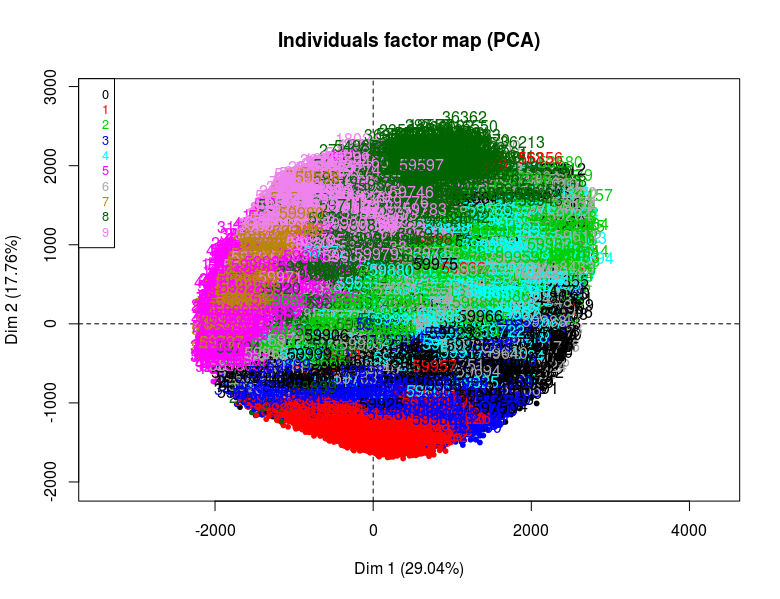
\includegraphics[width=300]{pca_ind_factor_map.png}
\caption{Plan factoriel des individus avec PCA.}
\label{fig:pca_ind}
\end{figure}

\begin{figure}[H] 
\centering
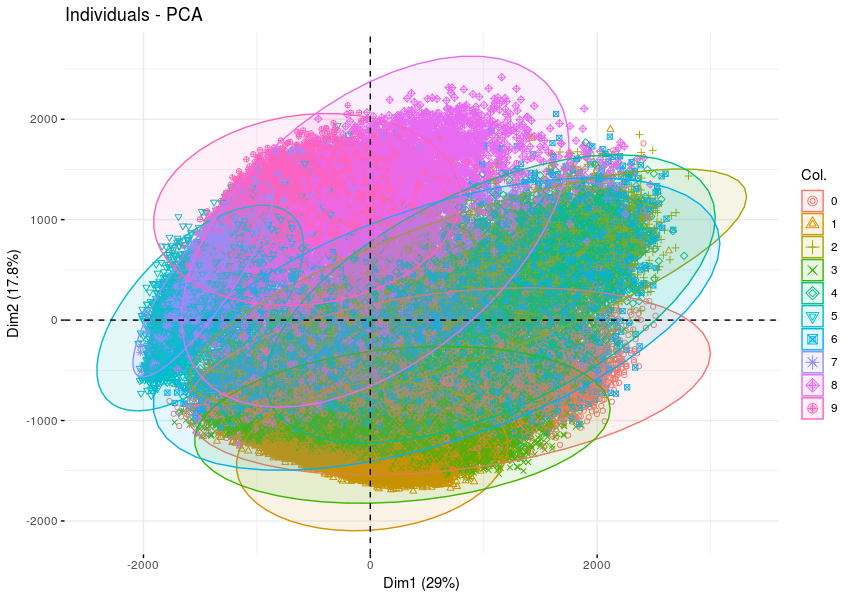
\includegraphics[width=\textwidth]{pca_ellipses.png}
\caption{Ellipse des classes avec PCA.}
\label{fig:pca_ellipse}
\end{figure}

On remarque sur la figure \ref{fig:pca_ellipse} que les clusters se confondent et semblent n'être pas sufisamment séparés sur les deux composantes principales du PCA. Cela fait sens avec le pourcentage de la variance expliquée par ces deux composantes (46.8\%).

Sur les figures suivantes nous voyons à gauche l'image reconstruite et à droite l'image originale pour chaque classe. Nous avons choisi les 50 premières composantes qui expliquent 86.27\% de la variance totale. Le choix du nombre de 50 s'est fait en affichant la variance totale expliquée pour chaque composante, c'est environ à ce chiffre que la variance augmente très lentement.

\begin{figure}[H] 
\centering
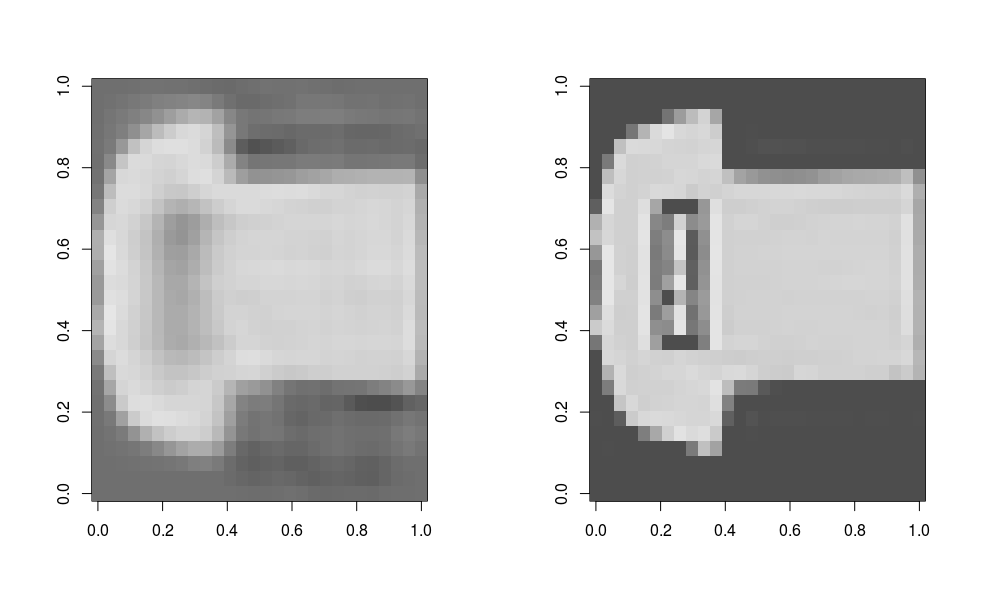
\includegraphics[width=\textwidth, trim=0 0 0 5cm]{pca_reconst_0.png}
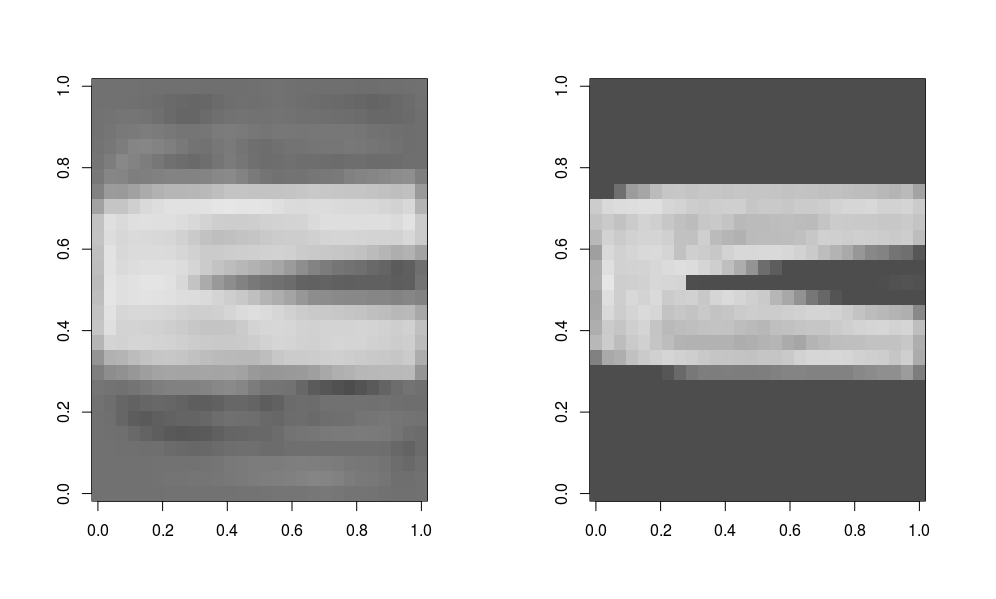
\includegraphics[width=\textwidth]{pca_reconst_1.png}
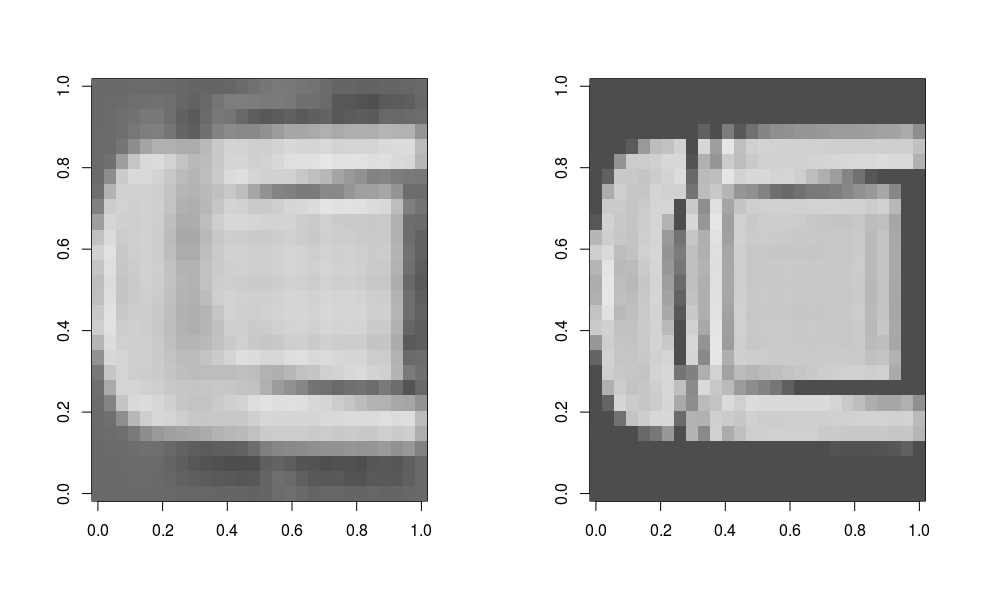
\includegraphics[width=\textwidth]{pca_reconst_2.png}
\label{fig:pca_ellipse}
\end{figure}

\begin{figure}[H] 
\centering
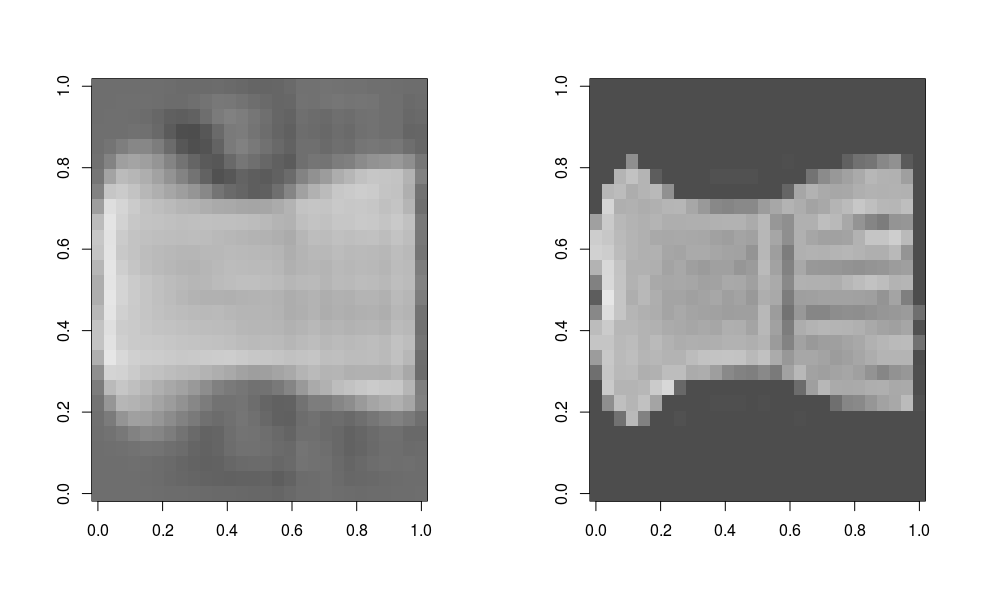
\includegraphics[width=\textwidth, trim=0 0 0 5cm]{pca_reconst_3.png}
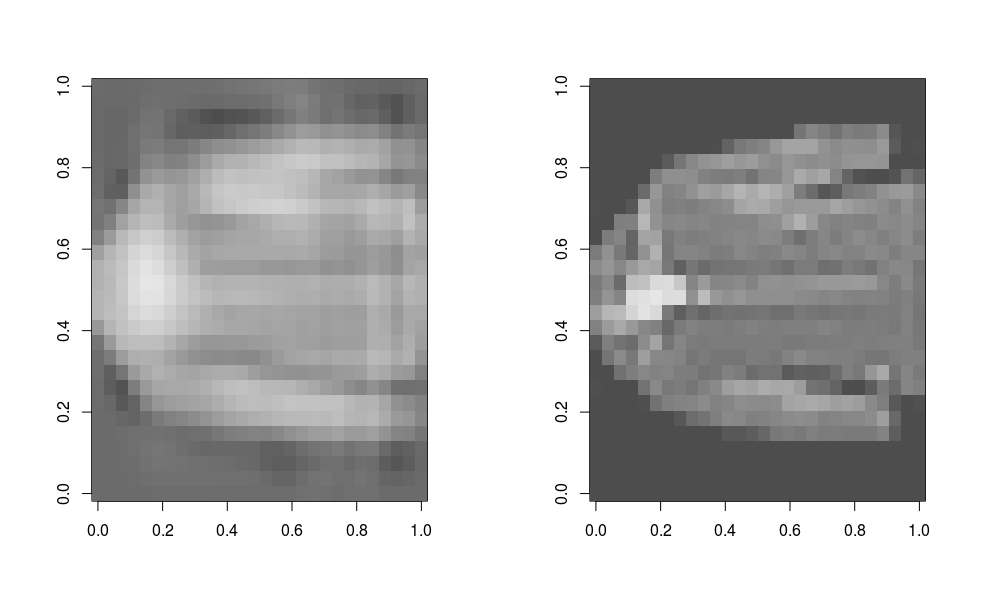
\includegraphics[width=\textwidth]{pca_reconst_4.png}
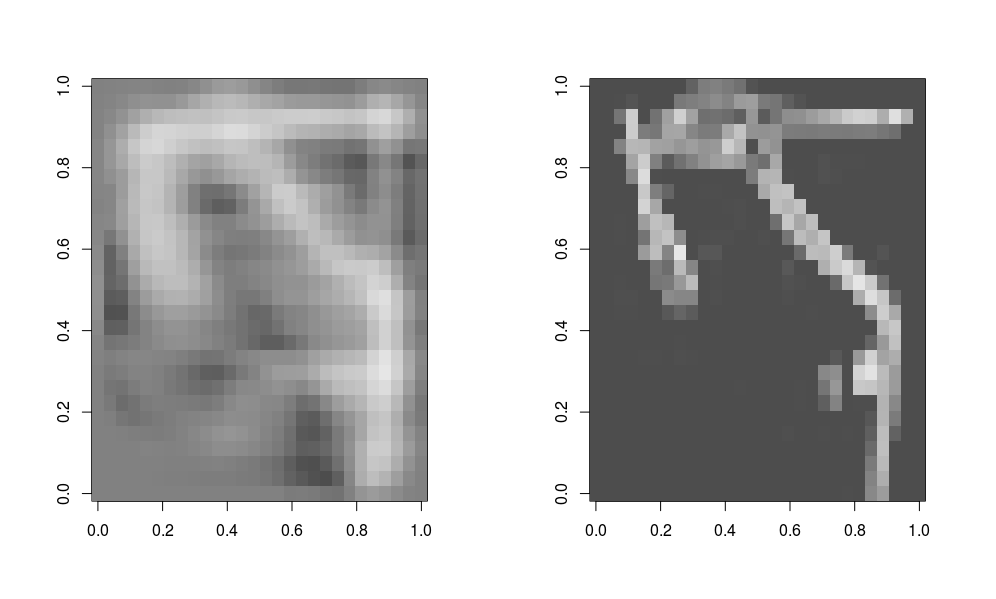
\includegraphics[width=\textwidth]{pca_reconst_5.png}
\label{fig:pca_ellipse}
\end{figure}

\begin{figure}[H] 
\centering
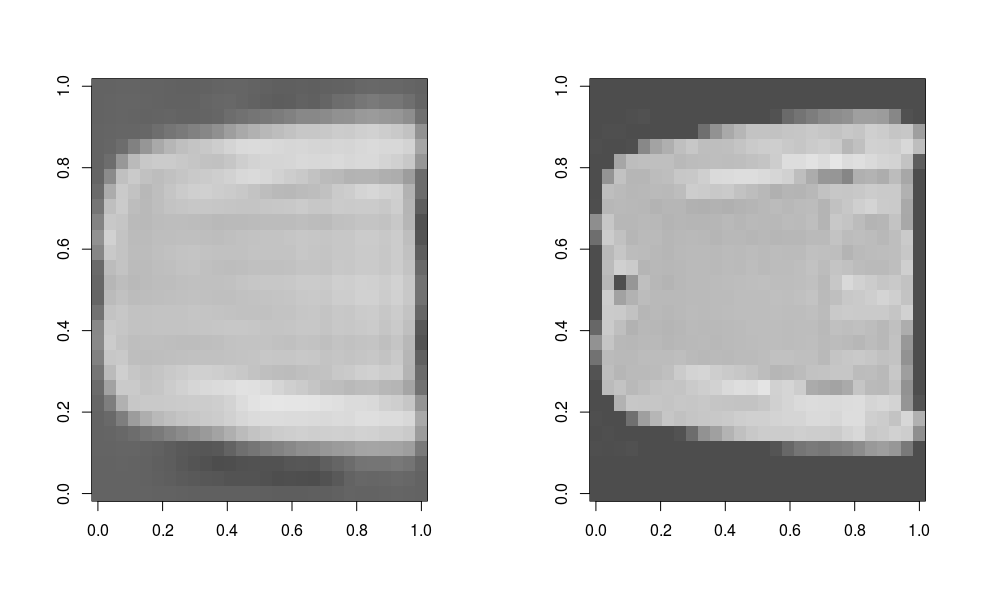
\includegraphics[width=\textwidth, trim=0 0 0 5cm]{pca_reconst_6.png}
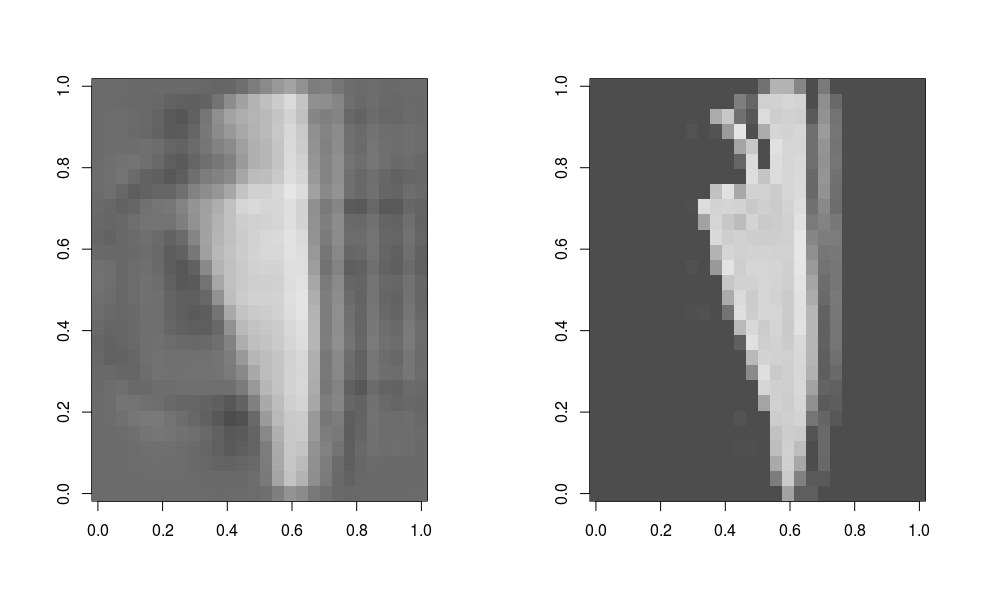
\includegraphics[width=\textwidth]{pca_reconst_7.png}
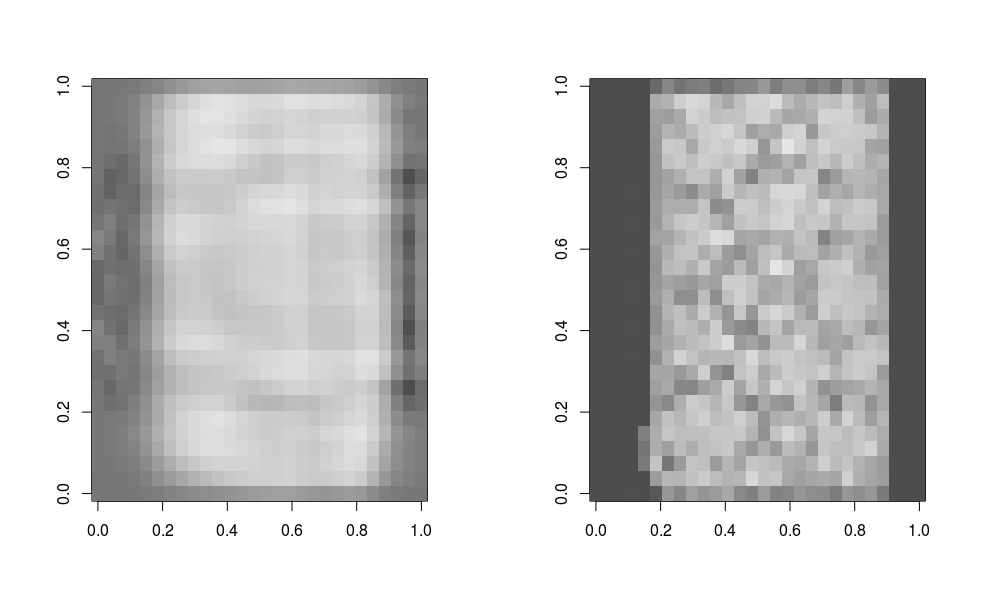
\includegraphics[width=\textwidth]{pca_reconst_8.png}
\label{fig:pca_ellipse}
\end{figure}

\begin{figure}[H] 
\centering
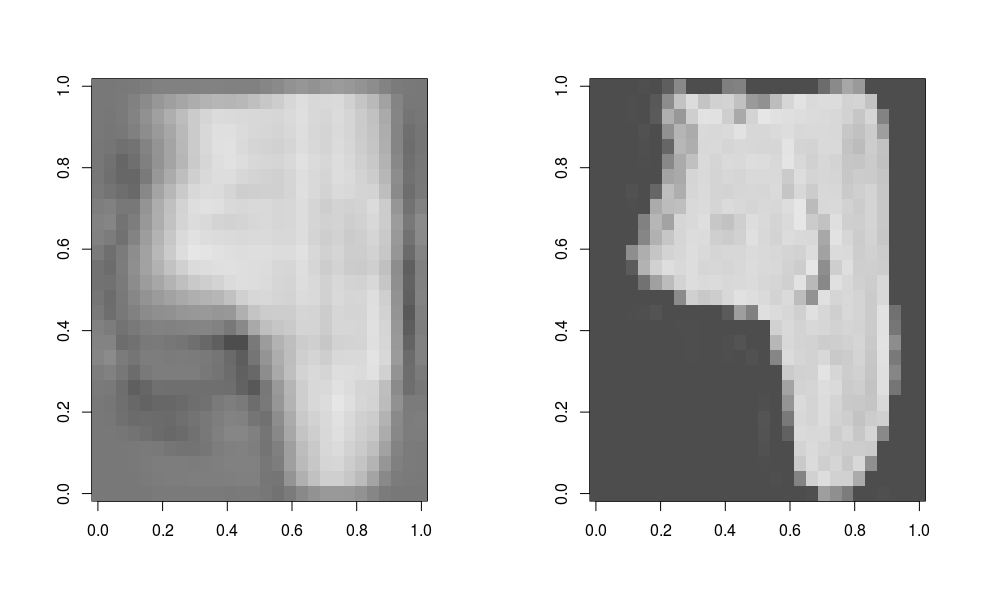
\includegraphics[width=\textwidth, trim=0 0 0 5cm]{pca_reconst_9.png}
\label{fig:pca_ellipse}
\end{figure}

\section{t-distributed Stochastic Neighbor Embedding (t-SNE)}

Après avoir étudier la documentation de la fonction TSNE de la librairie \textit{sklearn} pour python nous observons 3 principaux hyper-paramètres: \textit{perplexity}, \textit{early exaggeration} et \textit{learning rate}. 

La méthode nous donne en sortie la valeur de la divergence de Kullback-Leibler qui est une mesure de dissimilarité entre deux distributions, nous devons donc chercher les hyper-paramètres minimisant cette valeur le plus possible.

\section{Autoencoder}

\section{K-Means}

\section{Support Vector Machines (SVM)}

\section{Linear Discriminant Analysis (LDA)}

\section*{References}

\end{document}
